\section{Textual DSL}
\label{appendix.xtext}

\subsection{XText Grammar}

\begin{figure}[H]
    \begin{center}
        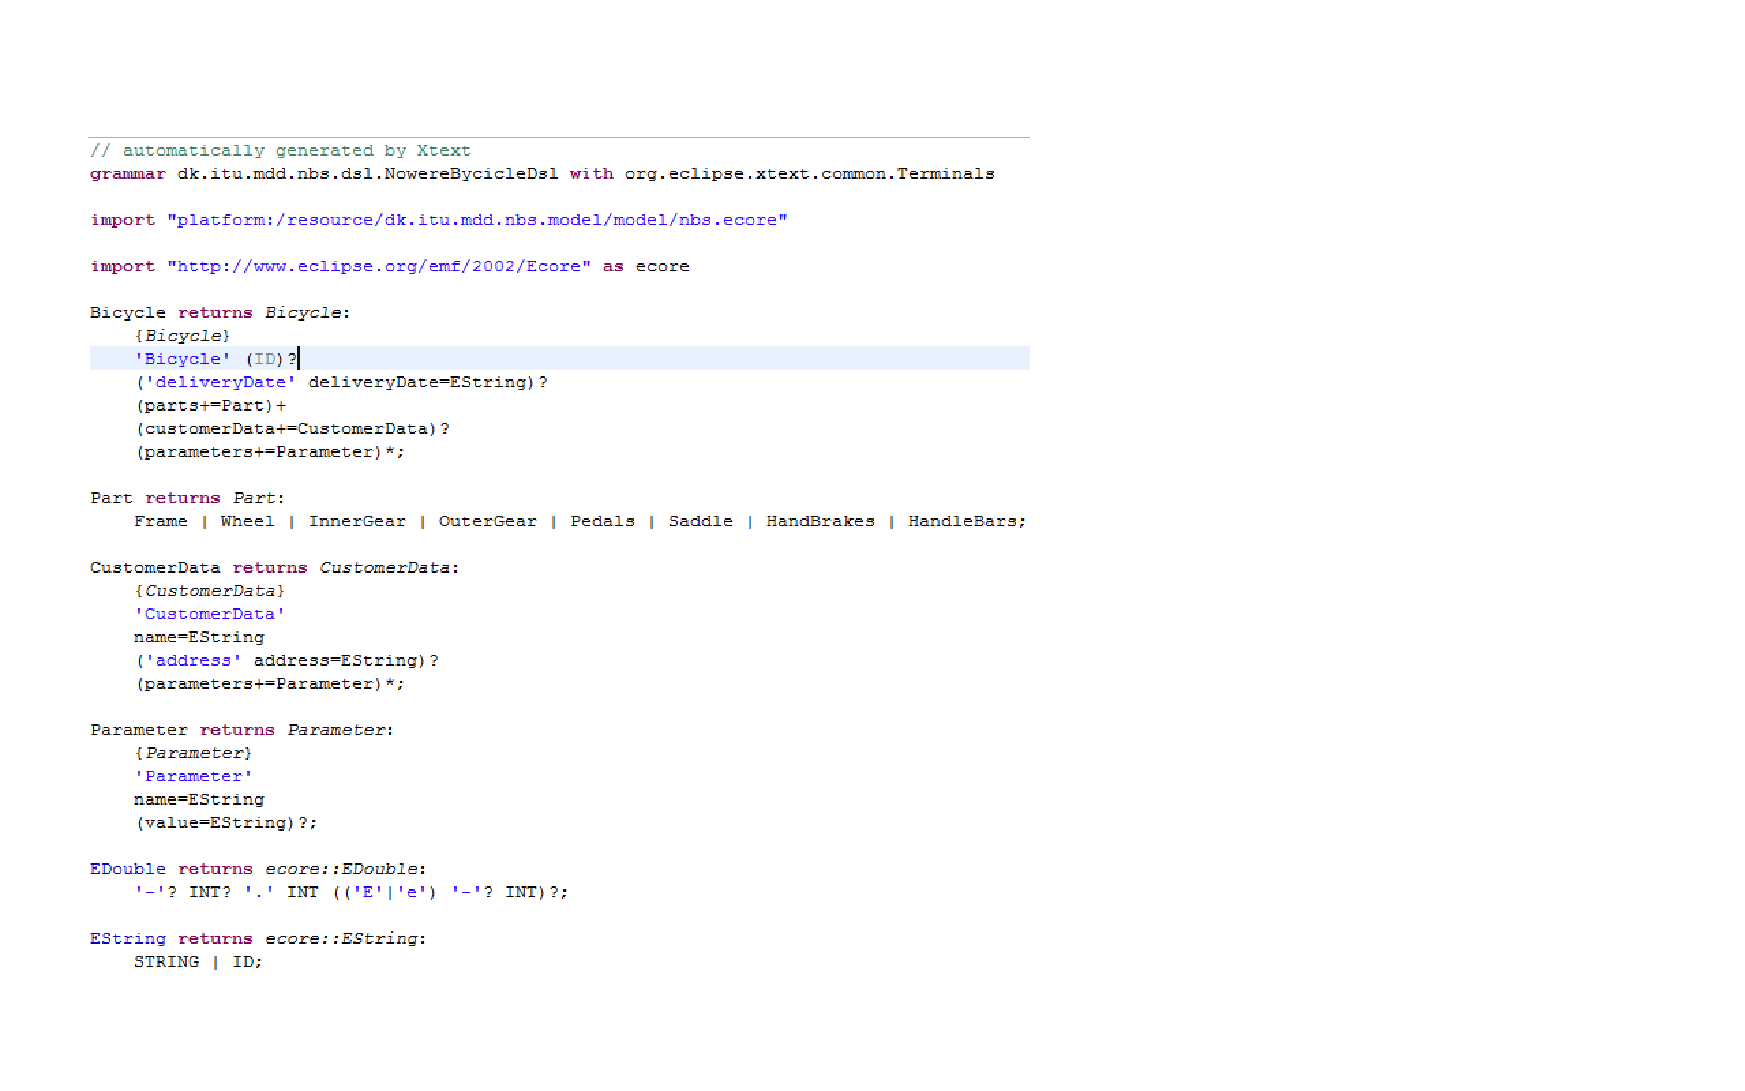
\includegraphics[width=\textwidth]{fig/xtext/grammar_1.pdf}
    \end{center}
\end{figure}

\begin{figure}[H]
    \begin{center}
        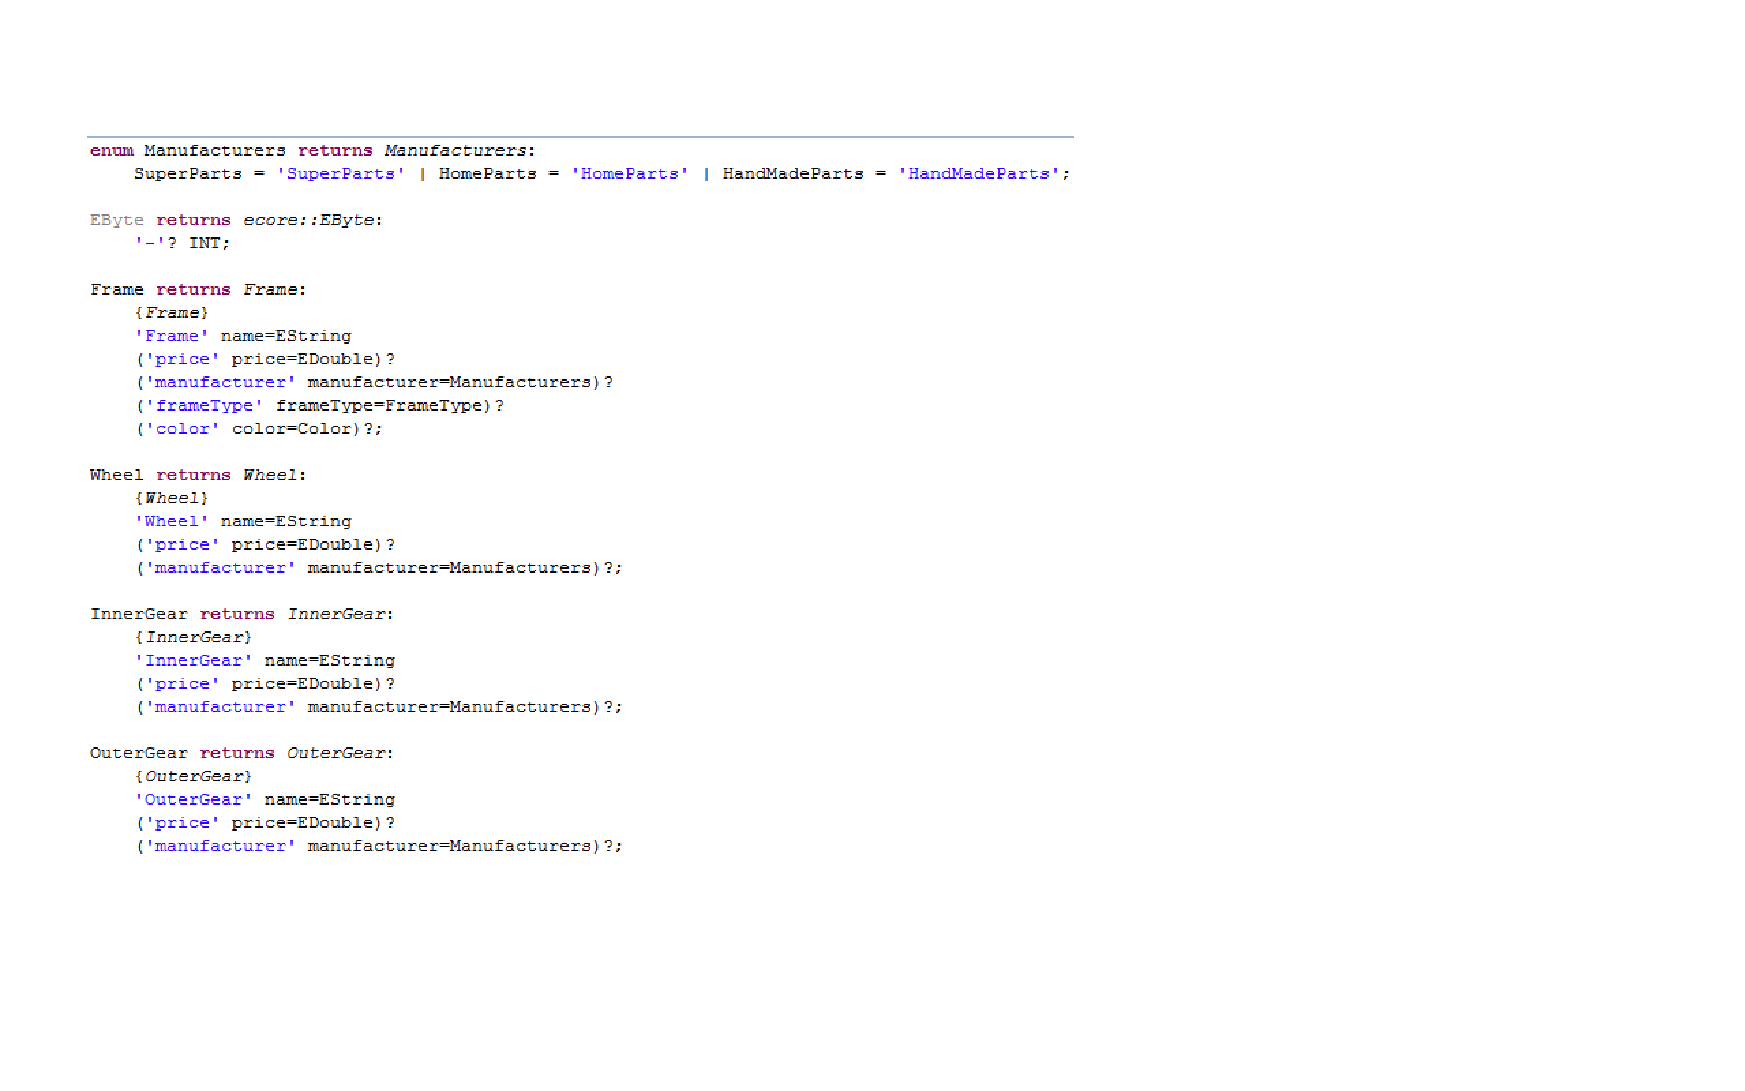
\includegraphics[width=\textwidth]{fig/xtext/grammar_2.pdf}
    \end{center}
\end{figure}

\begin{figure}[H]
    \begin{center}
        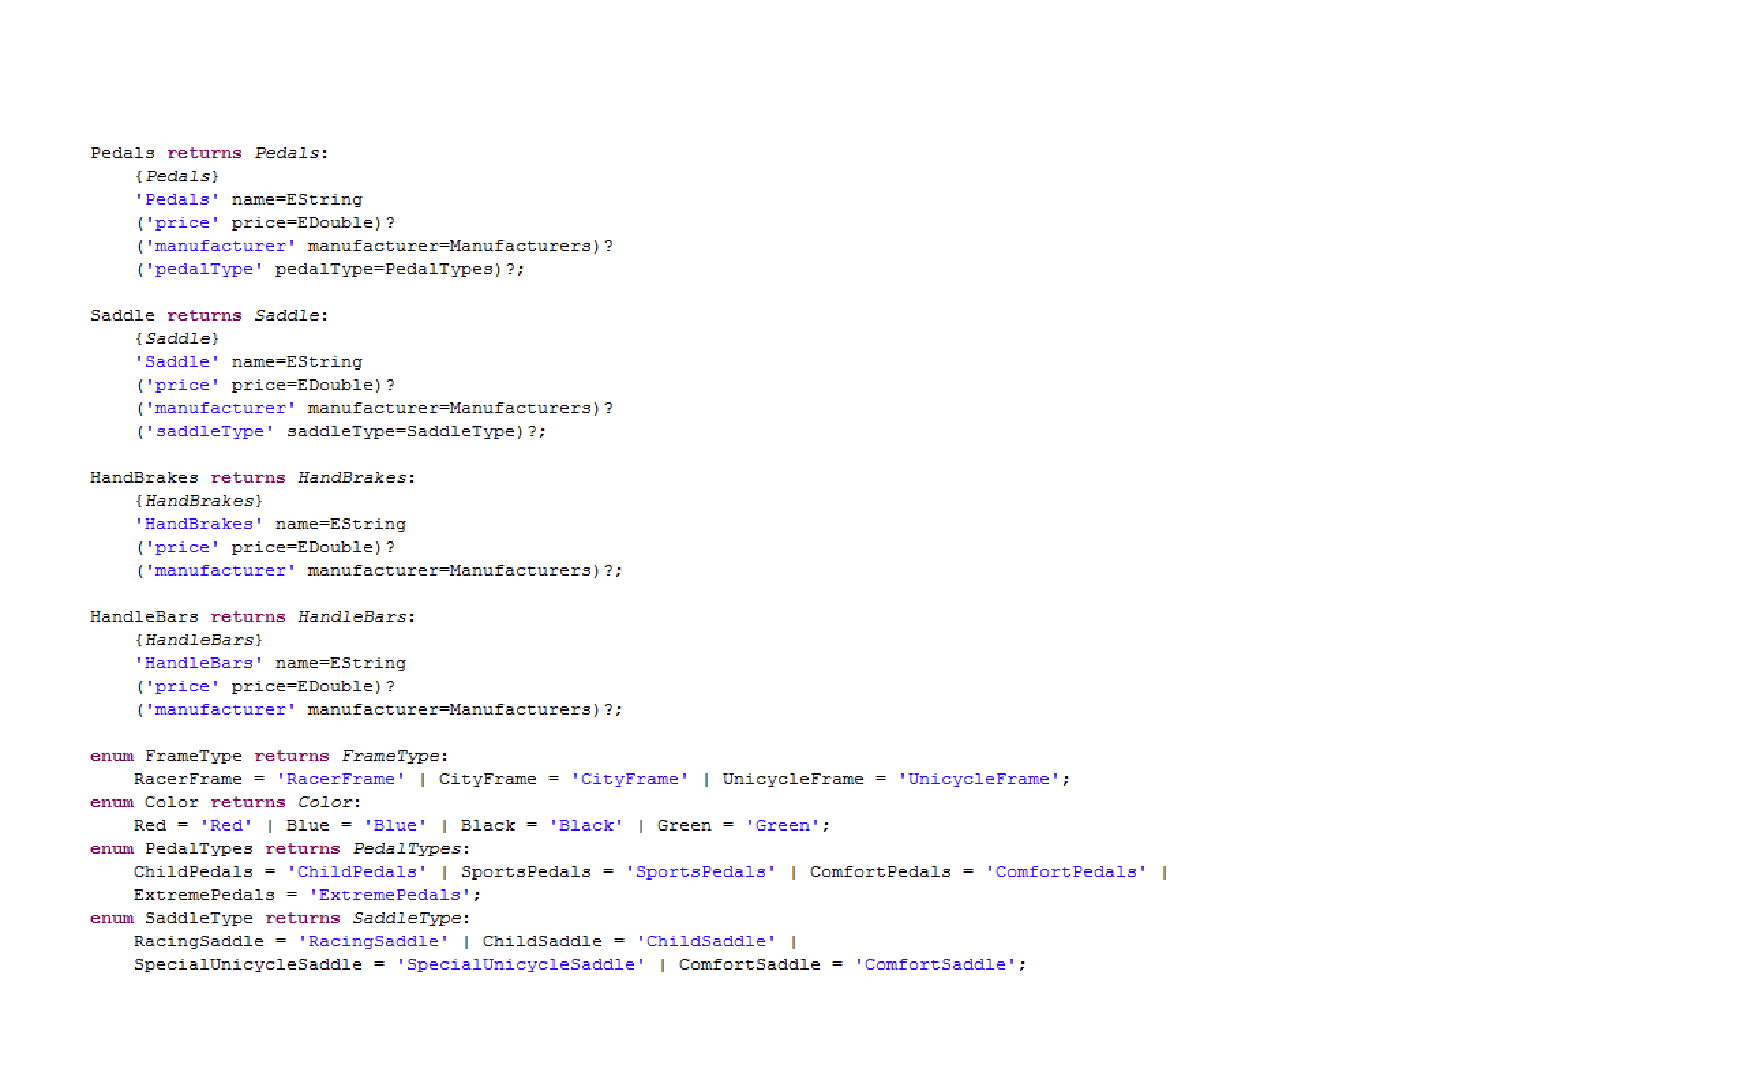
\includegraphics[width=\textwidth]{fig/xtext/grammar_3.pdf}
    \end{center}
\end{figure}

\subsection{Custom Bicycles modeled in Textual DSL}

\begin{figure}[H]
    \begin{center}
        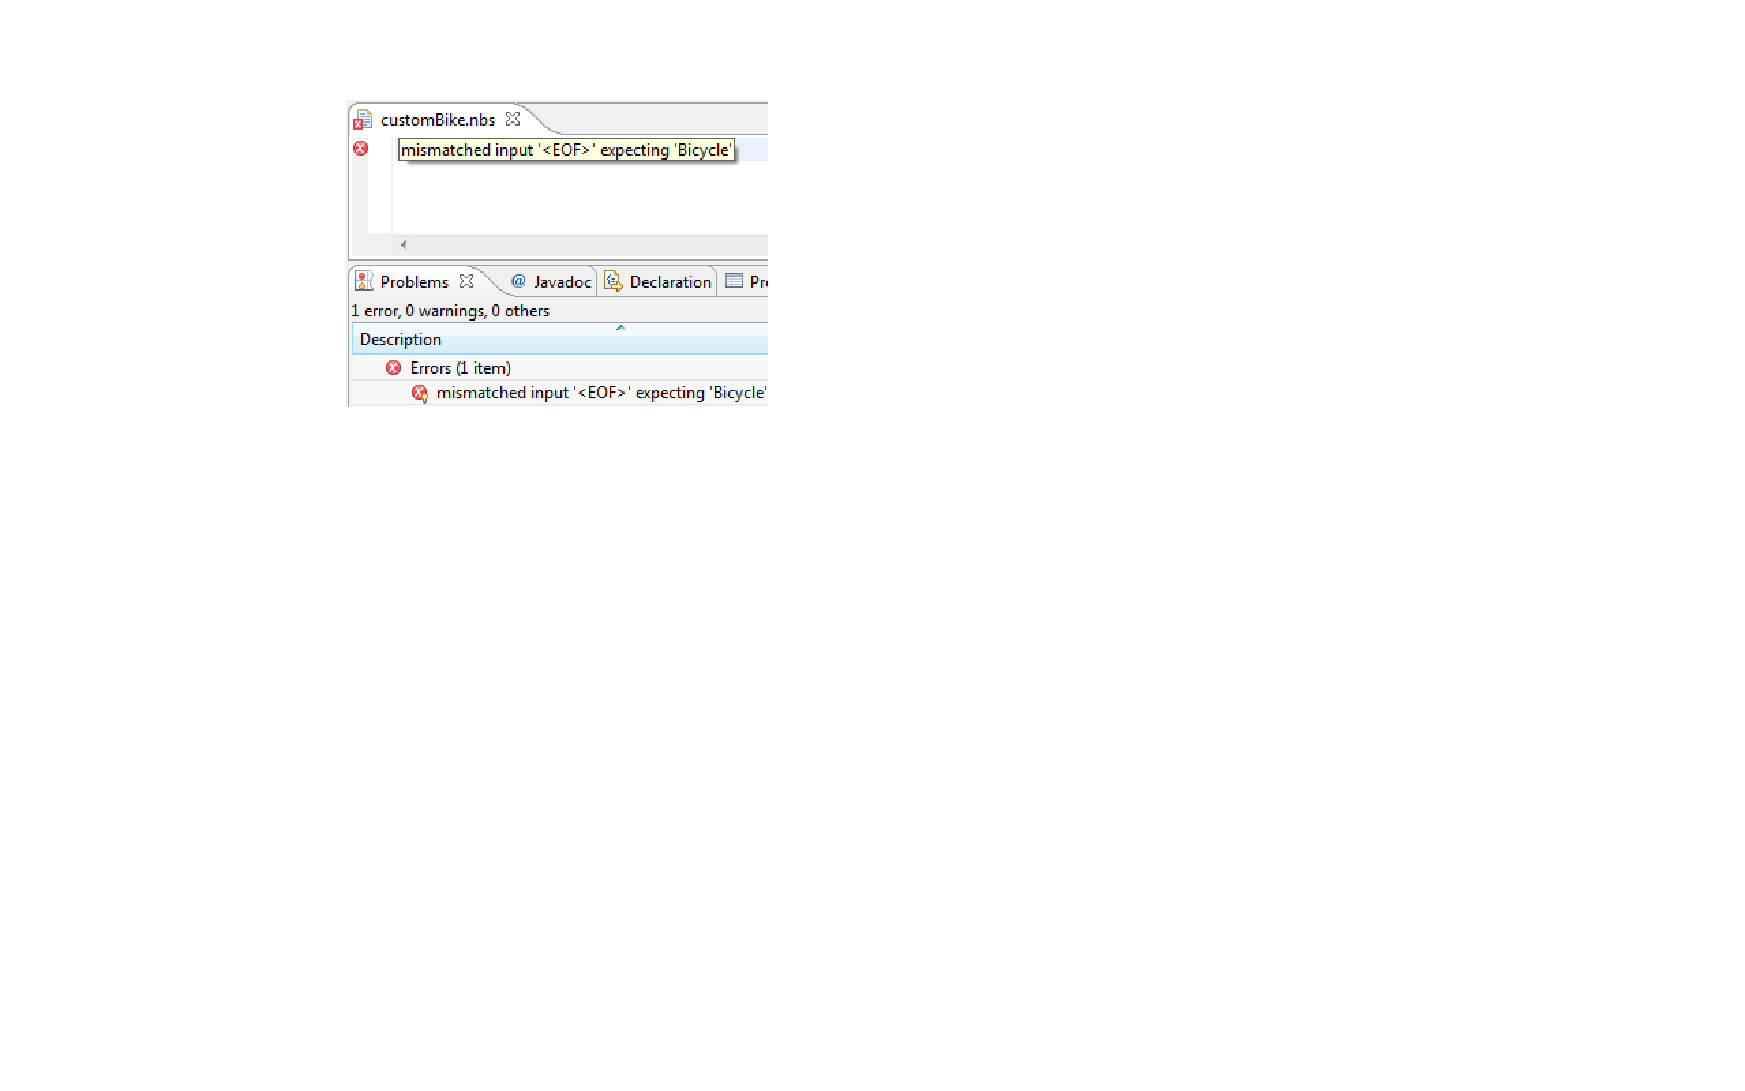
\includegraphics[width=\textwidth]{fig/xtext/xtext_example_empty_error.pdf}
        \caption{An empty bicycle model}
        \label{fig.dsl_empty_model}
    \end{center}
\end{figure}

\begin{figure}[H]
    \begin{center}
        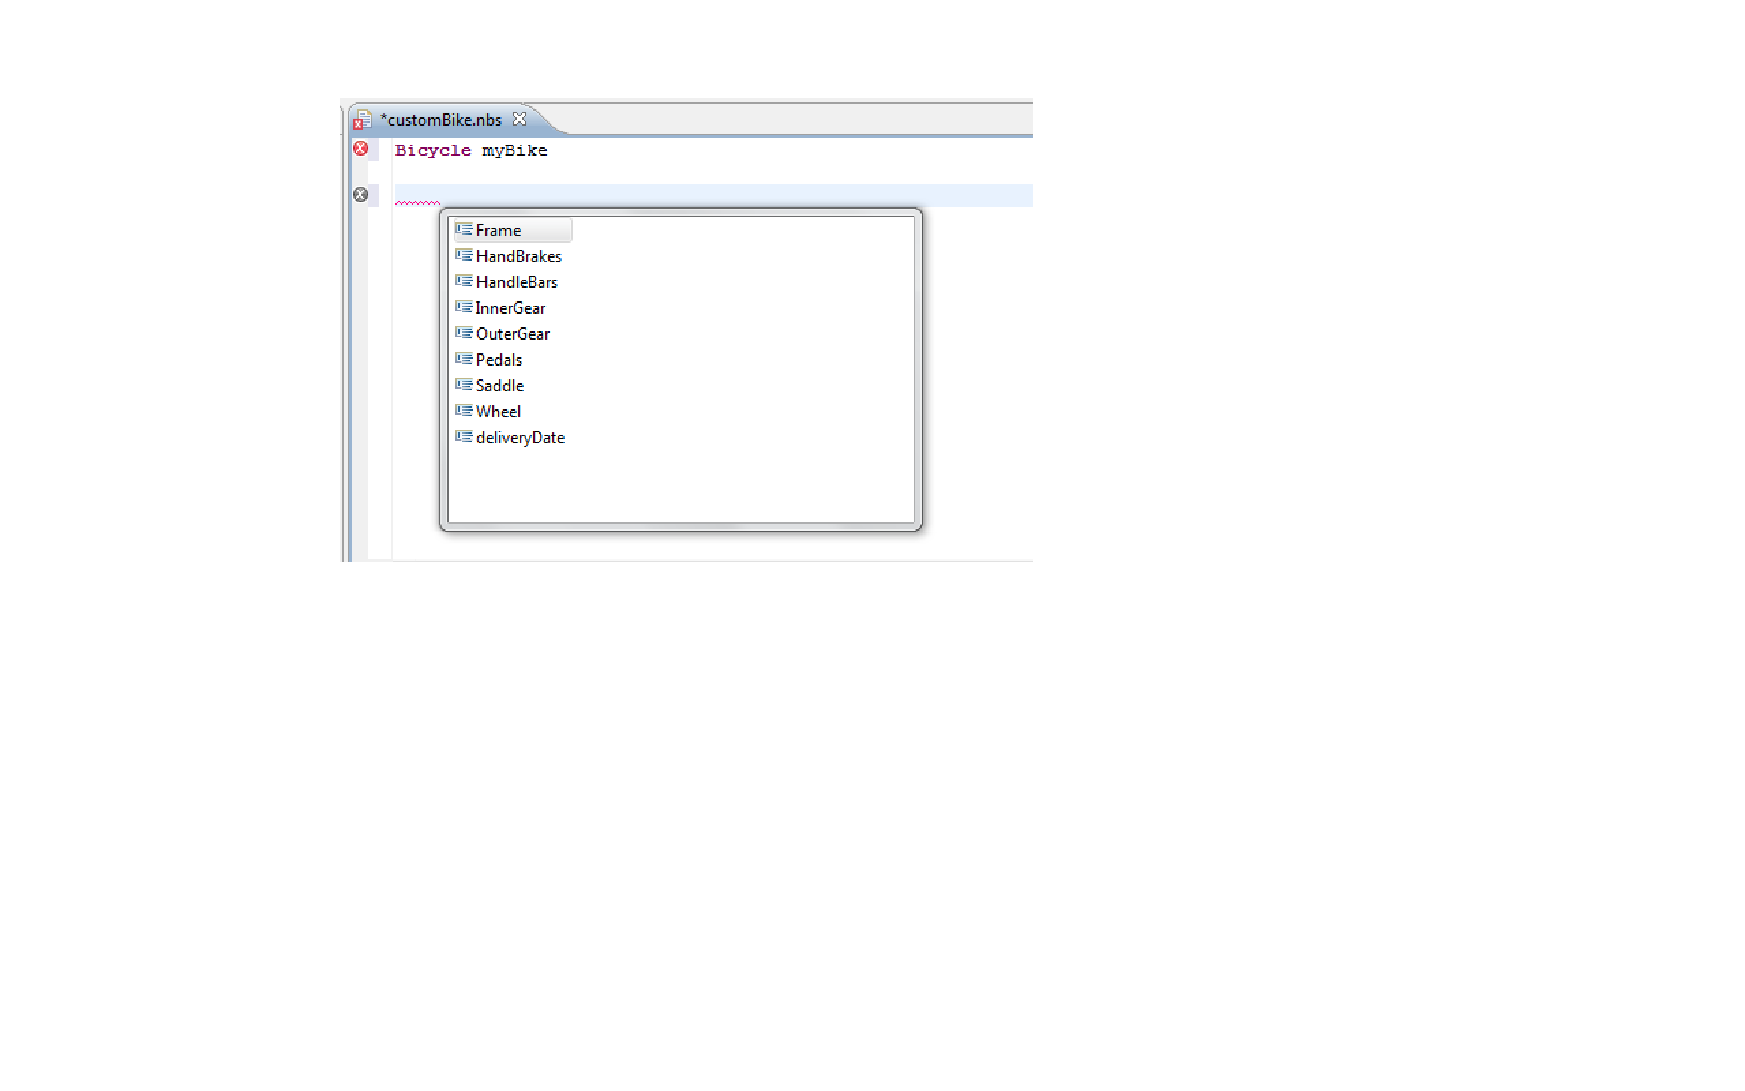
\includegraphics[width=\textwidth]{fig/xtext/xtext_example_autocomplete.pdf}
        \caption{Autocomplete support for Parts}
        \label{fig.dsl_autocomplete_parts}
    \end{center}
\end{figure}

\begin{figure}[H]
    \begin{center}
        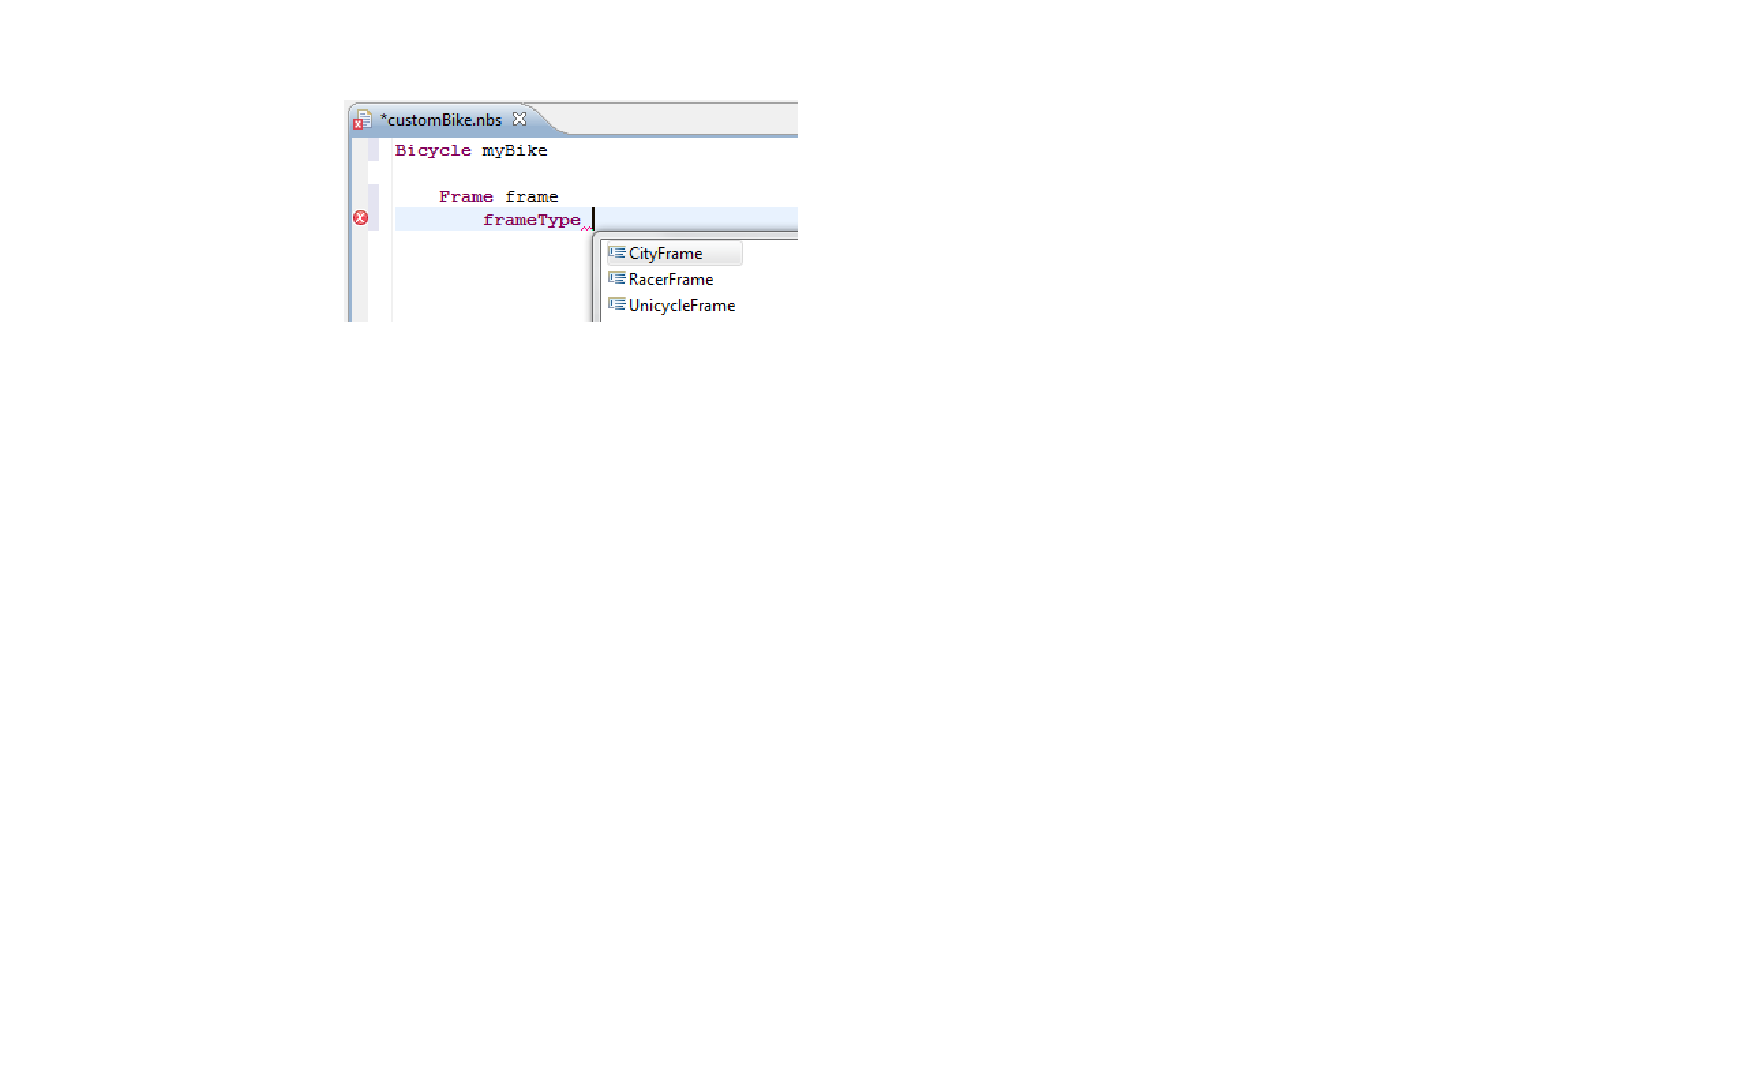
\includegraphics[width=\textwidth]{fig/xtext/xtext_example_autocomplete_value.pdf}
        \caption{Autocomplete support for possible values}
        \label{fig.dsl_autocomplete_values}
    \end{center}
\end{figure}

\begin{figure}[H]
    \begin{center}
        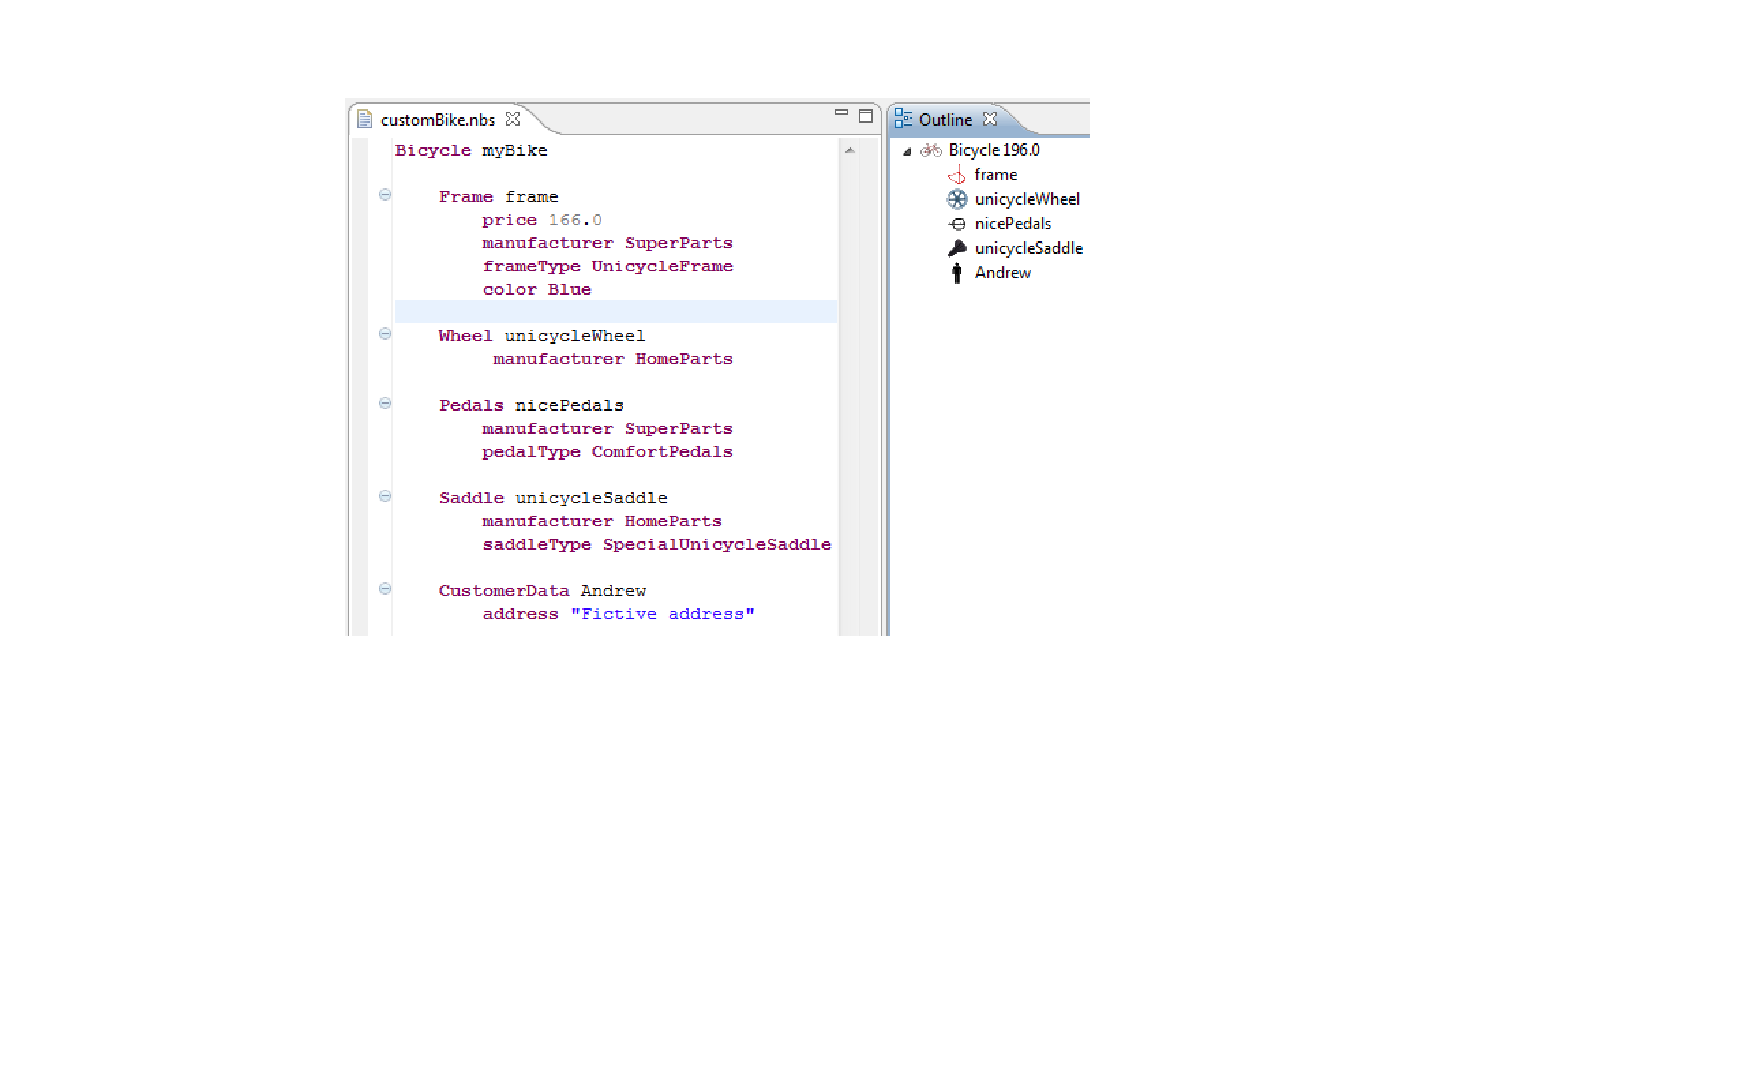
\includegraphics[width=\textwidth]{fig/xtext/xtext_example_complete.pdf}
        \caption{A complete bicycle model}
        \label{fig.dsl_complete}
    \end{center}
\end{figure}